\documentclass[presentation]{beamer}
\usetheme{metropolis}
\usepackage{polyglossia}
\setmainlanguage[variant=usmax]{english}
\usepackage{fontspec}
\usepackage{microtype}
\usepackage{geometry}
\usepackage{mathtools}
\usepackage[shortlabels]{enumitem}
\usepackage{graphicx}

\usepackage{tabulary}
\usepackage{booktabs}
\usepackage{multirow}

\usepackage{pgfplots}
\pgfplotsset{compat=newest}
\usepackage{tikz}
\usetikzlibrary{matrix,fit,backgrounds,calc,positioning,arrows.meta}

\author{Henrik Eide, Sondre Aasemoen}
\date{Spring 2022}
\title{INF236 Mandatory 3}
\begin{document}

\maketitle
\begin{frame}{Plan}
\tableofcontents
\end{frame}

\section{Introduction}

\begin{frame}{Introduction}
  \begin{itemize}
    \item Two people, two problems 
    \item Complexity not a linear increase based on team size
    \item Wrote parallel implementations of merge sort and the mandelbrot set
  \end{itemize}
\end{frame}

\section{Mandelbrot}

\begin{frame}
  \begin{figure}[htbp]
    \centering
    
\includegraphics[width=.9\linewidth]{./figures/mandelbrot.jpg}
    \caption{A proper mandelbrot visualization}
  \end{figure}
\end{frame}

\begin{frame}
  \begin{itemize}
    \item Based on algorithm from Wikipedia, written in C++ 
    \item Calculate pixel step size, loop over all pixels and assign a color 
    \item Tried implementing coloring over printing an ASCII-representation 
    \item Spoiler alert, didn't work out
    \item Unsure if coloring algorithm wrong, image writer or something else
  \end{itemize}
\end{frame}

\begin{frame}
  \begin{figure}[htbp]
    \centering
    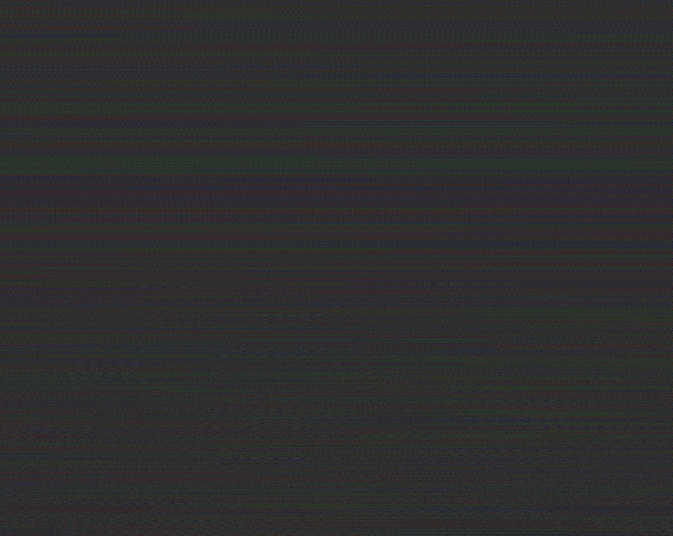
\includegraphics[width=.9\linewidth]{./figures/shittybrot.png}
    \caption{Our mandelbrot visualization}
  \end{figure}
\end{frame}

\begin{frame}
  \begin{table}[ht]
    \begin{tabulary}{.4\linewidth}{ rrr }
      \toprule
      Num threads & Runtime    & Speedup \\
      \midrule
      -           & 61.414685s  & 1 \\
      \midrule
      1           & 60.241224s  & 1.02 \\
      5           & 42.505744s  & 1.44 \\
      10          & 23.375631s  & 2.62  \\
      20          & 13.683191s  & 4.49  \\
      40          & 6.987723s  & 8.79 \\
      60          & 4.803215s & 12.79 \\
      80          & 3.813177s & 16.10 \\
      \bottomrule
    \end{tabulary}
    \caption{Results for mandelbrot}\label{table:mandel}
  \end{table}
\end{frame}

\begin{frame}
  \begin{figure}[ht]
    \centering
    \begin{tikzpicture}
      \begin{axis}[
        title={Runtime},
        xlabel={Number of threads},
        ylabel={Time in seconds},
        ymin=0, ymax=65,
        xmin=0, xmax=85,
        ymajorgrids=true,
        grid style=dashed,
        legend style={anchor=south east}
        ]
  
        \addplot[color=blue,mark=square*,line width=1pt]
        coordinates {
          (1,  61.414685)
          (5, 61.414685)
          (10, 61.414685)
          (20, 61.414685)
          (40, 61.414685)
          (60, 61.414685)
          (80, 61.414685)
        };
        \addplot[color=red,mark=square*,line width=1pt]
        coordinates {
          (1, 60.241224)
          (5, 42.505744)
          (10, 23.375631)
          (20, 13.683191)
          (40, 6.987723)
          (60, 4.803215)
          (80, 3.813177)
        };
        \legend{Seq, Par}
      \end{axis}
    \end{tikzpicture}
    \caption{Plot for runtime}
  \end{figure}
\end{frame}

\begin{frame}
  \begin{figure}[ht]
     \begin{tikzpicture}
      \begin{axis}[
        title={Speedup},
        xlabel={Number of threads},
        ylabel={Speedup},
        xmin=0, xmax=60,
        ymin=0, ymax=12,
        ytick={0,1,...,14},
        ymajorgrids=true,
        grid style=dashed,
        legend style={anchor=south east}
        ]

        \addplot[color=red,mark=square*,line width=1pt]
        coordinates {
          (1, 1.02)
          (5, 1.44)
          (10, 2.62)
          (20, 4.49 )
          (40, 8.79)
          (60, 12.79)
          (80, 16.10)
        };
        \addplot[color=blue,mark=square*,line width=1pt]
        coordinates { (1, 1 ) (5, 1 ) (10, 1 ) (20, 1 ) (40, 1 ) (60, 1 ) (80, 1) };
        \legend{Seq, Par}
      \end{axis}
    \end{tikzpicture}
    \caption{Plot for speedup}
  \end{figure}
\end{frame}

\section{Merge sort}

\begin{frame}
  \begin{itemize}
    \item Some stuff about merge sort
  \end{itemize}
\end{frame}

\section{Conclusion}

\begin{frame}{Mandelbrot}
  \begin{itemize}
    \item ``Embarrassingly parallel'' problem
    \item Near linear speed increase
    \item Main loop need no expensive synchronization, only adding data to image
    \item No need for guards, prefix sums etc.
    \item Thought it would be more complex than it actually was
  \end{itemize}
\end{frame}

\end{document}
